% !TeX root = relazione.tex
\documentclass{article}

\usepackage[utf8]{inputenc}
\usepackage[a4paper, total={15.3 cm, 21.3 cm}]{geometry}
\usepackage{amsmath}
\usepackage{amssymb}
\usepackage{gensymb}
\usepackage{booktabs}
\usepackage{hyperref}
\usepackage{caption}
\usepackage{float}
\usepackage{graphicx}
\usepackage{subfig}
\usepackage{titlesec}
\usepackage{titletoc}
\usepackage{physics}
\usepackage{siunitx}
\usepackage[dvipsnames]{xcolor}
\usepackage{longtable}
\usepackage{calc}
\usepackage{array}
\usepackage{subfiles} % Best loaded last in the preamble
\usepackage{etoolbox}
\usepackage{xparse}

\hypersetup{colorlinks=true,linkcolor=black}
\renewcommand\thesection{\arabic{section}}
\titlecontents{chapter}[1.05em]{\bigskip}
{\contentslabel[\MakeUppercase{\romannumeral\thecontentslabel}]{1em}\enspace\textsc}
{\hspace*{-1em}\textsc}
{\hfill\contentspage}
\titlecontents{section}[1.6em]{\smallskip}
{\thecontentslabel.\enspace}
{}
{\titlerule*[1pc]{.}\contentspage}
\setcounter{tocdepth}{2}


\begin{document}

    \pagenumbering{roman}
    \thispagestyle{empty}

    \begin{center}

        
\includegraphics[width=1.\linewidth]{../../tools/images/logo.jpg}
        \centering
        \vspace{3cm}

        {\uppercase{\Large Misura rapporto di $e/m $\par}}
        \vspace{3cm}

        {\Large Lorenzo Liuzzo, Jiahao Miao, Riccardo Salto\par}
        \vspace{1.5cm}

        {\Large Novembre 16, 2022}

    \end{center}
    \clearpage

    \tableofcontents
    \clearpage

    \pagenumbering{arabic}

\section{Abstract}
Avendo come scopo la misura del rapporto tra carica e massa dell'elettrone, è stato riprodotto l'esperimento di Thompson riadattandolo alle possibilità del laboratorio.
É stato osservato la scia fluorescente lasciata da un fascio di elettroni immerso in un campo magnetico approssimativamente uniforme in una ampolla di gas di idrogeno a bassa pressione(vedi figura \ref{fig:Bella}).
Conoscendo la geometria delle bobine e della corrente che la attraversa è possibile calcolare il campo magnetico generato dal sistema di bobine.
Dalla conoscenza dei valori di campo magnetico a cui è soggetto il fascio di elettroni, della differenza di potenziale che accelera il fascio di elettroni e del raggio dell'orbita circolare si risale al rapporto $e/m$.

Il miglior valore ottenuto è: 
    \[e/m = (1.76\pm0.06)10^{11}\frac{C}{kg}\]
\\

\begin{figure}[h]
    \centering
    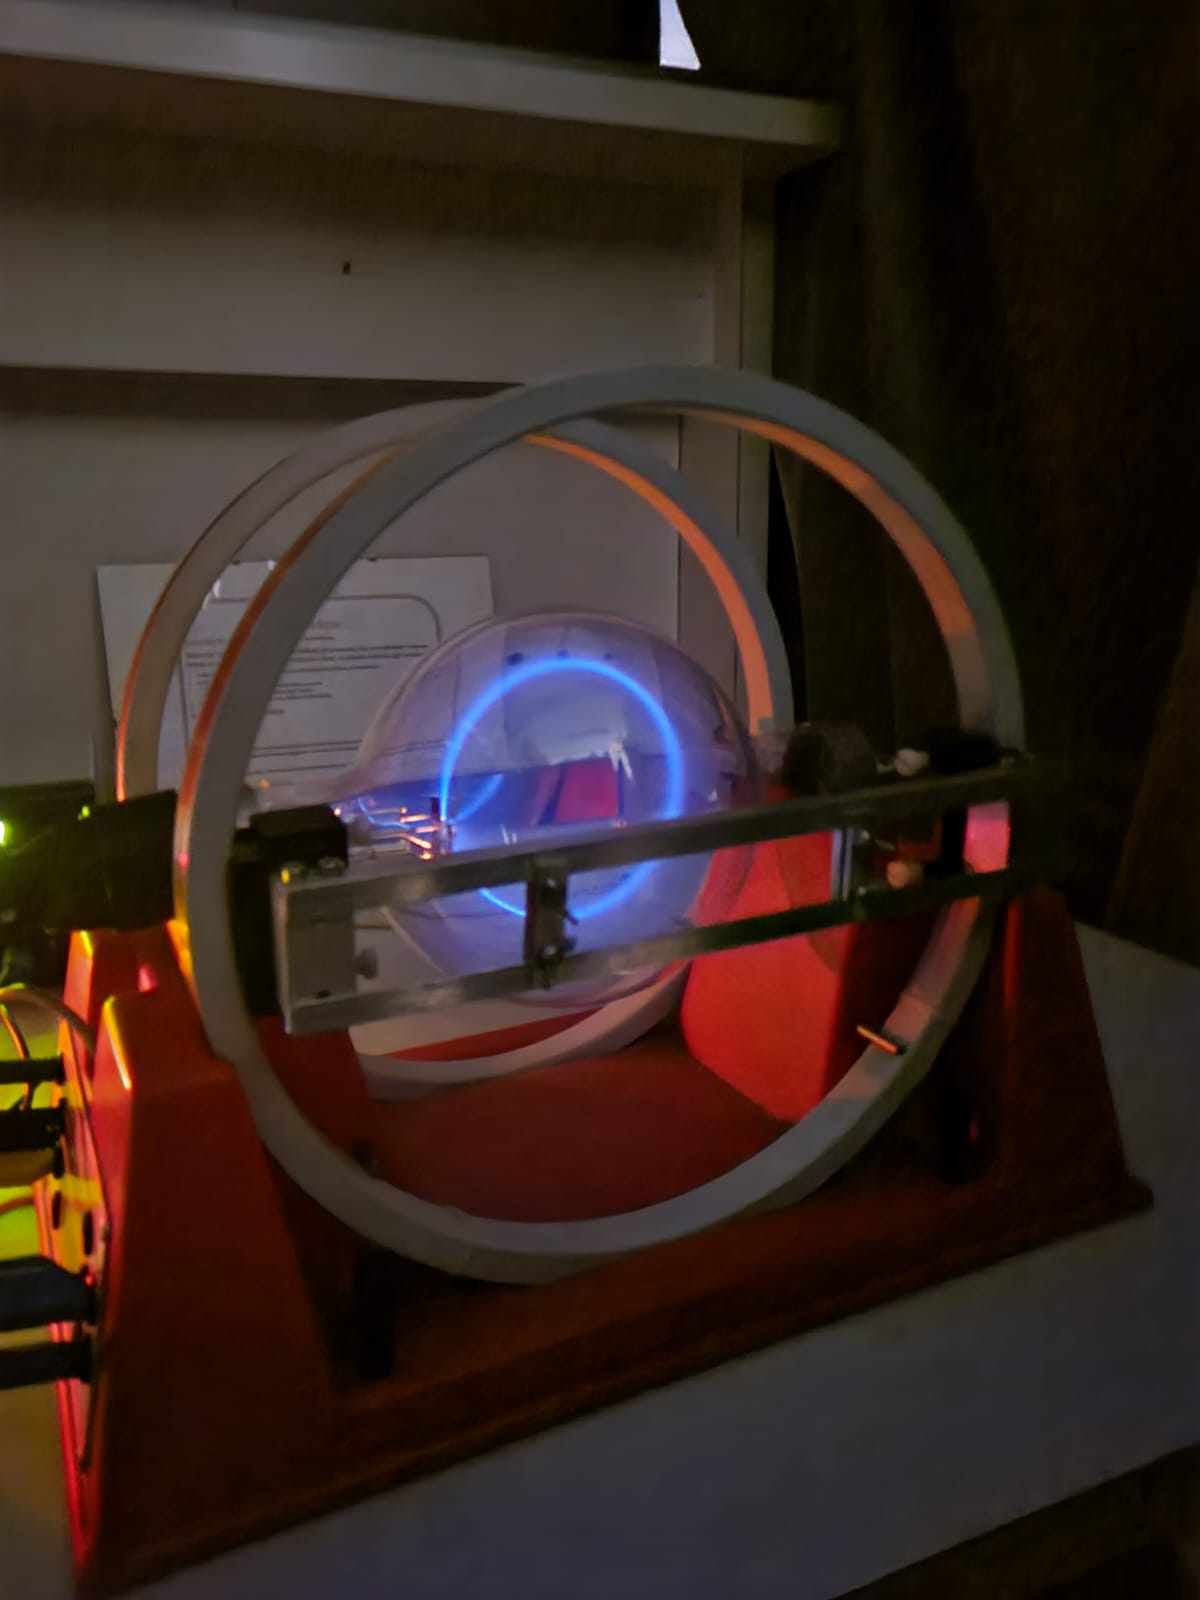
\includegraphics[scale=0.25,height= 9cm,width = 7 cm ]{../images/Apparato_sperimentale.jpeg}
    \caption{Traccia lasciata da un fascio di elettroni soggetto alla forza di Lorentz}
    \label{fig:Bella}
\end{figure}

\section{Metodi}
\subsection{Calibrazione Apparato} 
     Dopo aver collegato l'apparato ai generatori e ai due multimetri, è stata misurata con un calibro digitale la distanza tra le due bobine che in configurazione di Helmholtz è uguale al raggio delle stesse. Per questa misura è stata fatta una media tra la distanza esterna e quella interna. 
    \[ r_b = 0,157 \qq{m}\]
     A questo punto sono state spente le luci per rendere più visibile il fascio luminoso. Si è poi fissato il traguardo sinistro sulla guida in modo che coincidesse con il fascio; questo sarebbe poi rimasto in quella configurazione per tutta la durata dell'esperimento. Per limitare gli errori è stato posizionato a turno da tutti i componenti del gruppo di lavoro, con l'ausilio dello specchio per evitare gli effetti di parallasse. Una volta fissato, è stata fatta una stima dell'errore sulla misura del raggio: ogni elemento del gruppo ha riportato una misura dello stesso diametro (quindi a differenza di potenziale e intensità fissate) e da questi è stata calcolata la deviazione standard che è stata usata come errore di ogni misura per tutto l'arco dell'esperimento.
     \[\sigma_r = 2 \qq{mm}\]
     Prima di iniziare con le misurazioni in senso proprio, è stata verificata la seguente configurazione prendendo tre misure di prova e ottenendo così un valore indicativo di e/m = $1,72\cdot 10^{11}$ che è rientrato nel range di valori attesi ed è stato tra l'altro utilizzato nelle regressioni lineari per spostare gli errori nelle ascisse sulle ordinate. 
    
\subsection{Presa Dati}
    Il primo set di misure effettuate è stato in configurazione perpendicolare al campo magnetico terrestre. Sono state prese 10 misure di diametro per altrettante variazioni di differenza di potenziale e intensità di corrente (quindi campo magnetico generato dalle bobine). Per ognuno dei valori ottenuti è stato calcolato un valore indicativo di $e/m$ dalla relazione:
        \[ e/m = \frac{2\Delta V}{(B_z R)^2}\]
    Dove $\Delta V$ è la differenza di potenziale, $B_z$ è il modulo del campo magnetico indotto dalle bobine, $R$ è il raggio delle bobine. Il valore del campo magnetico è stato ricavato dalla relazione: 
        \[B_z=\delta \frac{8\mu_0 N I }{5\sqrt{5} R_b}\]
    Dove $\mu_0$ è la permeabilità magnetica nel vuoto, $N$ il numero di spire delle bobine e $R_b$ il raggio delle stesse e $\delta$ il fattore di correzione tabulato. L'errore associato $\sigma_{B_z}$ è stato ottenuto dalla seguente formula di propagazione:
    \[\sigma_{B_z} = \delta B_z \sqrt{(\frac{\sigma_I}{I})^2 + (\frac{\sigma_{R_b}}{R_b})^2}\]
    Dove $\sigma_I$ è l'errore associato all'intensità di corrente e $\sigma_{R_b}$ quello associato al raggio delle bobine.
    La procedura è stata ripetuta 3 volte, ponendo inizialmente l'apparato in modo che il campo magnetico terrestre fosse perpendicolare al campo magnetico indotto dalle bobine. Tenendo fissati il voltaggio e l'intensità di corrente è stato fatto ruotare l'apparato e si è verificato il verso del campo magnetico terrestre in base alla dilatazione o restrizione dell'orbita. A questo punto sono stati registrati altri due set di misure, uno in configurazione parallela, l'altro in configurazione antiparallela, aspettandosi rispettivamente una sovrastima e una sottostima del raggio delle orbite. Di seguito sono riportati per ogni misura il valore della differenza di potenziale applicata $\Delta V$, al quale è stato associato un errore di $0.1$ Volt pari alla risoluzione del generatore; il raggio dell'orbita percorsa dagli elettroni $R$ la cui incertezza di $0.002$m è stata stimata in fase di calibrazione; il valore dell'intensità di corrente $I$, con errore associato $0.001$A pari alla risoluzione dello strumento, il valore del campo magnetico indotto $B_z$ con l'errore associato $\sigma_{B_z}$, il valore associato di $e/m$ calcolato dalla relazione esposta nel paragrafo precedente (non è stato calcolato il singolo errore poiché la misura effettiva è stata effettuata tramite regressione lineare). In tabella \ref{misure ortogonali} i dati ricavati in configurazione perpendicolare, in tabella \ref{misure paralleli} quelli presi con campo terrestre parallelo a quello dell'apparato e in \ref{misure antiparalleli} sono riportati i dati relativi alla configurazione antiparallela. 
    
     \begin{table}[H]
   
    \centering
        \begin{tabular}{ cccccc } 
            \toprule 
         $\Delta V$[V] & $R$[m] & $I$[A] & $B_z$[T] & $\sigma_{B_z}$[T] & $e/m$[C kg$^{-1}$] \\
            \midrule 
            155,3	&	0,0510	&	1,024	&	0,000758	&	3E-06	&	2,08E+11\\
            179,1	&	0,0545	&	1,024	&	0,000757	&	3E-06	&	2,11E+11\\
            215,2	&	0,0610	&	1,025	&	0,000754	&	3E-06	&	2,03E+11\\
            245,2	&	0,0635	&	1,025	&	0,000752	&	3E-06	&	2,15E+11\\
            194,3	&	0,0590	&	1,029	&	0,000758	&	3E-06	&	1,94E+11\\
            165,3	&	0,0535	&	1,029	&	0,000761	&	4E-06	&	2,00E+11\\
            303,0	&	0,0540	&	1,370	&	0,001013	&	5E-06	&	2,03E+11\\
            224,4	&	0,0560	&	1,197	&	0,000884	&	4E-06	&	1,83E+11\\
            153,8	&	0,0450	&	1,208	&	0,000897	&	4E-06	&	1,89E+11\\
            191,3	&	0,0495	&	1,208	&	0,000895	&	4E-06	&	1,95E+11\\
            \bottomrule           
        \end{tabular}
        \caption{presa dati con apparato in configurazione ortogonale rispetto al campo magnetico terrestre}
        \label{misure ortogonali}
   \end{table}
   \begin{table}[H]
            \centering
            \begin{tabular}{ cccccc } 
            \toprule 
            $\Delta V$[V] & $R$[m] & $I$[A] & $B_z$[T] & $\sigma_{B_z}$[T] & $e/m$ [C kg^{-1}] \\
            \midrule 
            221,2	&	0,0490	&	1,277	&	0,000946	&	4E-06	&	2,06E+11\\
            125,1	&	0,0445	&	1,018	&	0,000756	&	3E-06	&	2,21E+11\\
            261,1	&	0,0600	&	1,162	&	0,000854	&	4E-06	&	1,99E+11\\
            374,9	&	0,0545	&	1,553	&	0,001147	&	5E-06	&	1,92E+11\\
            191,8	&	0,0550	&	1,102	&	0,000814	&	4E-06	&	1,91E+11\\
            280,0	&	0,0580	&	1,276	&	0,000940	&	4E-06	&	1,89E+11\\
            308,3	&	0,0585	&	1,318	&	0,000971	&	4E-06	&	1,91E+11\\
            159,2	&	0,0535	&	1,017	&	0,000752	&	3E-06	&	1,97E+11\\
            199,8	&	0,0470	&	1,307	&	0,000969	&	4E-06	&	1,92E+11\\
            193,5	&	0,0435	&	1,384	&	0,001028	&	5E-06	&	1,94E+11\\
            \bottomrule           
        \end{tabular}
        \caption{presa dati con apparato in configurazione parallela rispetto al campo magnetico terrestre}
        \label{misure paralleli}
    \end{table}
    \begin{table}[H]
        
            \centering
            \begin{tabular}{ cccccc } 
            \toprule 
            $\Delta V$[V] & $R$[m] & $I$[A] & $B_z$[T] & $\sigma_{B_z}$[T] & $e/m$[C kg^{-1}] \\
            \midrule 
            271,0	&	0,0620	&	1,230	&	0,000904	&	4E-06	&	1,72E+11    \\
            329,4	&	0,0600	&	1,396	&	0,001028	&	5E-06	&	1,73E+11    \\
            235,6	&	0,0500	&	1,395	&	0,001034	&	5E-06	&	1,76E+11    \\
            165,8	&	0,0630	&	0,924	&	0,000679	&	3E-06	&	1,81E+11    \\
            182,7	&	0,0660	&	0,924	&	0,000677	&	3E-06	&	1,83E+11    \\
            120,4	&	0,0540	&	0,925	&	0,000684	&	3E-06	&	1,77E+11    \\
            221,6	&	0,0415	&	1,582	&	0,001175	&	5E-06	&	1,86E+11    \\
            359,2	&	0,0580	&	1,542	&	0,001137	&	5E-06	&	1,65E+11    \\
            252,0	&	0,0610	&	1,235	&	0,000909	&	4E-06	&	1,64E+11    \\
            462,0	&	0,0525	&	1,854	&	0,001372	&	6E-06	&	1,78E+11    \\
            \bottomrule           
        \end{tabular}
        \caption{presa dati con apparato in configurazione antiparallela rispetto al campo magnetico terrestre}
        \label{misure antiparalleli}
    \end{table}
    
    Con i dati raccolti è stato utilizzato il metodo dei minimi quadrati per trovare il valore migliore di $e/m$ con la sua incertezza per ogni set. La relazione lineare utilizzata è:
    \begin{equation}\label{Relazione lineare}
        (B_z R)^2 = m/e (2\Delta V) 
    \end{equation}
        
    Per le tre configurazioni, perpendicolare, parallela e antiparallela, sono stati ricavati rispettivamente i tre valori con $\chi$ quadro associato:
    \begin{align*}
        e/m_{ort} &= (2,1 \pm 0,2)\cdot 10^{11} \qq{C/Kg} \quad \chi^2 = 51\% \\
        e/m_{par} &= (1,63 \pm 0,08) \cdot 10^{11} \qq{C/Kg} \quad \chi^2 = 94\% \\
        e/m_{ant} &= (1,7 \pm 0,1) \cdot 10^{11}  \qq{C/Kg} \quad \chi^2 = 30\%
    \end{align*}

    Il test del $\chi^2$ è stato eseguito per verificare la compatibilità dei dati con la relazione lineare \ref{Relazione lineare} e risultano tutti compatibili con una distribuzione lineare.
   
       
    GRAFICI REGRESSIONI

    

\subsection{Misura del campo magnetico terrestre}
    Al fine di operare una correzione sui valori ottenuti, è stato misurato il campo magnetico terrestre osservando gli spostamenti angolari di un ago magnetico in presenza e in assenza di un campo magnetico indotto con delle bobine. Il modulo del campo magnetico terrestre è stato ricavato dalla relazione:\\
    \[B_t = \frac{I}{I_0}(B_z\cot(\theta)+B_r\]
    Dove
    \begin{itemize}
        \item $I$ è la corrente imposta dal generatore di corrente, $I_0$ è la corrente di riferimento pari a 100 mA
        \item $\theta$ è l'angolo segnato dalla bussola
        \item $B_z$ e $B_r$ sono rispettivamente le componenti nella direzione dell'asse delle bobine e del Nord magnetico.
    \end{itemize}
    In tabella \ref{tab:B tabulati} sono riportati i valori tabulati di $B_z$ e $B_r$ riferiti ad una corrente $I_0$ di 100 mA.

    \begin{table}[h]
        \centering            
            \begin{tabular}{ccc}
            \toprule
            $\theta$ [°] & $B_z$ [G] & $B_r$ [mG] \\ 
            \midrule
            10 & 1,4750 & 20,9 \\ 
            20 & 1,4951 & 34,2 \\ 
            30 & 1,5190 & 36,2 \\ 
            40 & 1,5379 & 28,6 \\ 
            70 & 1,5423 & 0,1 \\ 
            \bottomrule
        \end{tabular}
        \caption{Valori Tabulati di $B_z$ e $B_r$}
        \label{tab:B tabulati} 
    \end{table}

Nella tabella \ref{tab:orario e antiorario} sono riportate gli angoli, che corrispondono a quelli della tabella \ref{tab:B tabulati} convertiti in radianti, l'intensità di corrente $I$ e il corrispondente valore di campo magnetico terrestre $B_t$. 
        \begin{table}[h]
        \centering
        \begin{tabular}{ c c c c c c}
            \toprule
            $\theta$[rad] & $\sigma_\theta$[rad] & I[mA] & $\sigma_I$[mA] & $B_t$[G] & $B_t$[G] \\
            \midrule
            0,17 & 0,02 & 6 & 1 & 0,482 & 0,090 \\ 
            0,35 & 0,02 & 12 & 1 & 0,484 & 0,045 \\ 
            0,52 & 0,02 & 18 & 1 & 0,487 & 0,030 \\ 
            0,70 & 0,02 & 27 & 1 & 0,510 & 0,022 \\ 
            1,22 & 0,02 & 89 & 1 & 0,500 & 0,018 \\ 
            \bottomrule
        \end{tabular}
        \caption{Misure in senso orario e antiorario}
        \label{tab:orario e antiorario}
    \end{table}

    Si nota subito nella tabella \ref{tab:orario e antiorario} che l'incertezza sulla corrente è molto elevata, si è ritenuto necessario assegnargli questa incertezza poiché il multimetro non dava una lettura stabile del valore.
    Inoltre, gli stessi valori della corrente sono stati osservati per portare la lancetta della bussola allo stesso angolo, ma in antiorario.

    Con una media pesata è stato ricavato il valore $B_t$ utilizzato per le correzioni:
    \[B_t = (5.0\pm 0.1)\cdot10^{-5}T\]
    

\section{Analisi dati}
    Utilizzando il valore del campo magnetico terrestre precedentemente misurato, sono state corrette le relazioni:
    \begin{align*}
        e/m&= \frac{2\Delta V}{((B_z+B_t)R)^2}  \qq{Parallelo}\\
        e/m &= \frac{2\Delta V}{((B_z-B_t)R)^2} \qq{Anti-Parallello}
    \end{align*}
    A questo punto sono state rifatte tutte le regressioni lineari e sono stati ottenuti i tre valori finali per le tre rispettive configurazioni:
        \begin{align*}
            e/m_{ort}&=(2,1 \pm 0,2) \cdot 10^{11} \qq{C/Kg} \\
            e/m_{par} &= (1,5 \pm 0,1) \cdot 10^{11} \qq{C/Kg} \\
            e/m_{ant} &= (1,78 \pm 0,08) \cdot 10^{11} \qq{C/Kg}
        \end{align*}
    Questi valori dovrebbero essere la misura di una singola grandezza, ma come si può osservare sono differenti tra di loro. Dunque prima di procedere con la media pesata si è eseguito un test di compatibilità con il valore medio pari a $1.84\cdot10^{11}$ e deviazione standard pari a $0.22\cdot10^{11}$

    Il test è risultato ha portato come risultato:
    \[\chi^2 = 2.00 \quad \Tilde{\chi}^2= \frac{\chi^2}{1} = 2.00 \qq{e} P(\Tilde{\chi}^2 \ge 2.00) = 16\% \]

    Ciò vuol dire che ripetendo lo stesso esperimento ci sarebbe il $37\%$ di trovare risultati peggiori di questi, nell'ipotesi che le misure siano governate secondo una distribuzione Gaussiana con valore medio la media dei tre valori. Basandoci su questa evidenza, possiamo affermare che i valori sono compatibili tra di loro.
    
    Si è quindi ottenuto un unico valore attraverso una media pesata:
    \[e/m= (1.67\pm0.05)\cdot 10^{11}\frac{C}{kg}\]
    Combinando questo risultato con i risultati dell'esperimento di Millikan è stata ricavata la massa dell'elettrone con errore relativo ricavato dalla somma in quadratura degli errori relativi delle due grandezze:
    \[m_e=(9.6\pm 0.3)10^{-31}kg\]
    
\section{Considerazioni finali}
    La prima cosa che si osserva dalle misure è che sono tutte leggermente sovrastimate. Questo errore sistematico è probabilmente dovuto all'apparato che non è in perfette condizioni. 

\end{document}